\begin{frame}{SOAP: un sobre XML y un contrato WSDL}
\begin{columns}[c]
\begin{column}{0.4\textwidth}
\centering
\begin{tikzpicture}[sobre/.style={draw=verde,thick,rounded corners=3pt,align=center,font=\small}]
\node[sobre,minimum width=4.6cm,minimum height=4.0cm,fill=verdesuave] (env) {};
\node[anchor=north west,font=\small\bfseries,color=verde] at ([xshift=4pt,yshift=-3pt]env.north west) {Envelope};
\node[sobre,minimum width=4.0cm,minimum height=0.7cm,fill=white] (hdr) at ([yshift=-1.0cm]env.north) {Header (seguridad, etc.)};
\node[sobre,minimum width=4.0cm,minimum height=1.9cm,fill=white] (body) at ([yshift=1.25cm]env.south) {};
\node[anchor=north west,font=\small\bfseries,color=verde] at ([xshift=4pt,yshift=-2pt]body.north west) {Body};
\node[font=\scriptsize,align=center] at ([yshift=-0.2cm]body.center) {operación y datos\\o un \texttt{Fault} si falla};
\end{tikzpicture}
\end{column}
\begin{column}{0.56\textwidth}
\begin{itemize}
\item El WSDL describe operaciones, mensajes y dirección del servicio \cite{w3c_wsdl11}.
\item Cada mensaje es un sobre XML que viaja por HTTP POST \cite{w3c_soap12}.
\item En el SRI, la operación \texttt{validarComprobante} recibe la factura en XML codificado en base64 \cite{sri_recepcion}.
\end{itemize}
\end{column}
\end{columns}
\end{frame}

\begin{frame}{REST: recursos, verbos HTTP y JSON}
\begin{columns}[c]
\begin{column}{0.5\textwidth}
\begin{itemize}
\item Cada recurso tiene una URI propia \cite{fielding2000}.
\item Los verbos tienen significado: \texttt{GET} lee, \texttt{POST} crea, \texttt{PUT} reemplaza, \texttt{DELETE} borra \cite{rfc9110}.
\item El servidor no guarda estado entre peticiones y las respuestas pueden ir a caché \cite{fielding2000}.
\item El contrato es opcional: OpenAPI \cite{openapi31}.
\end{itemize}
\end{column}
\begin{column}{0.46\textwidth}
\begin{block}{Petición real en nuestro PFC}
\scriptsize
\texttt{GET /api/estado/solicitud/1}\\
\texttt{Authorization: Bearer <JWT>}\\[4pt]
\texttt{200 OK}\\
\texttt{\{"solicitudId":1,}\\
\texttt{\ "solicitudEstado":"APROBADA",}\\
\texttt{\ "anteproyectoEstado":"ENVIADO",}\\
\texttt{\ "actaGenerada":false, ...\}}
\end{block}
\end{column}
\end{columns}
\end{frame}

\begin{frame}{Arquitectura: los dos estilos en nuestro PFC}
\centering
\IfFileExists{../diagrama/arquitectura-servicios-web.png}{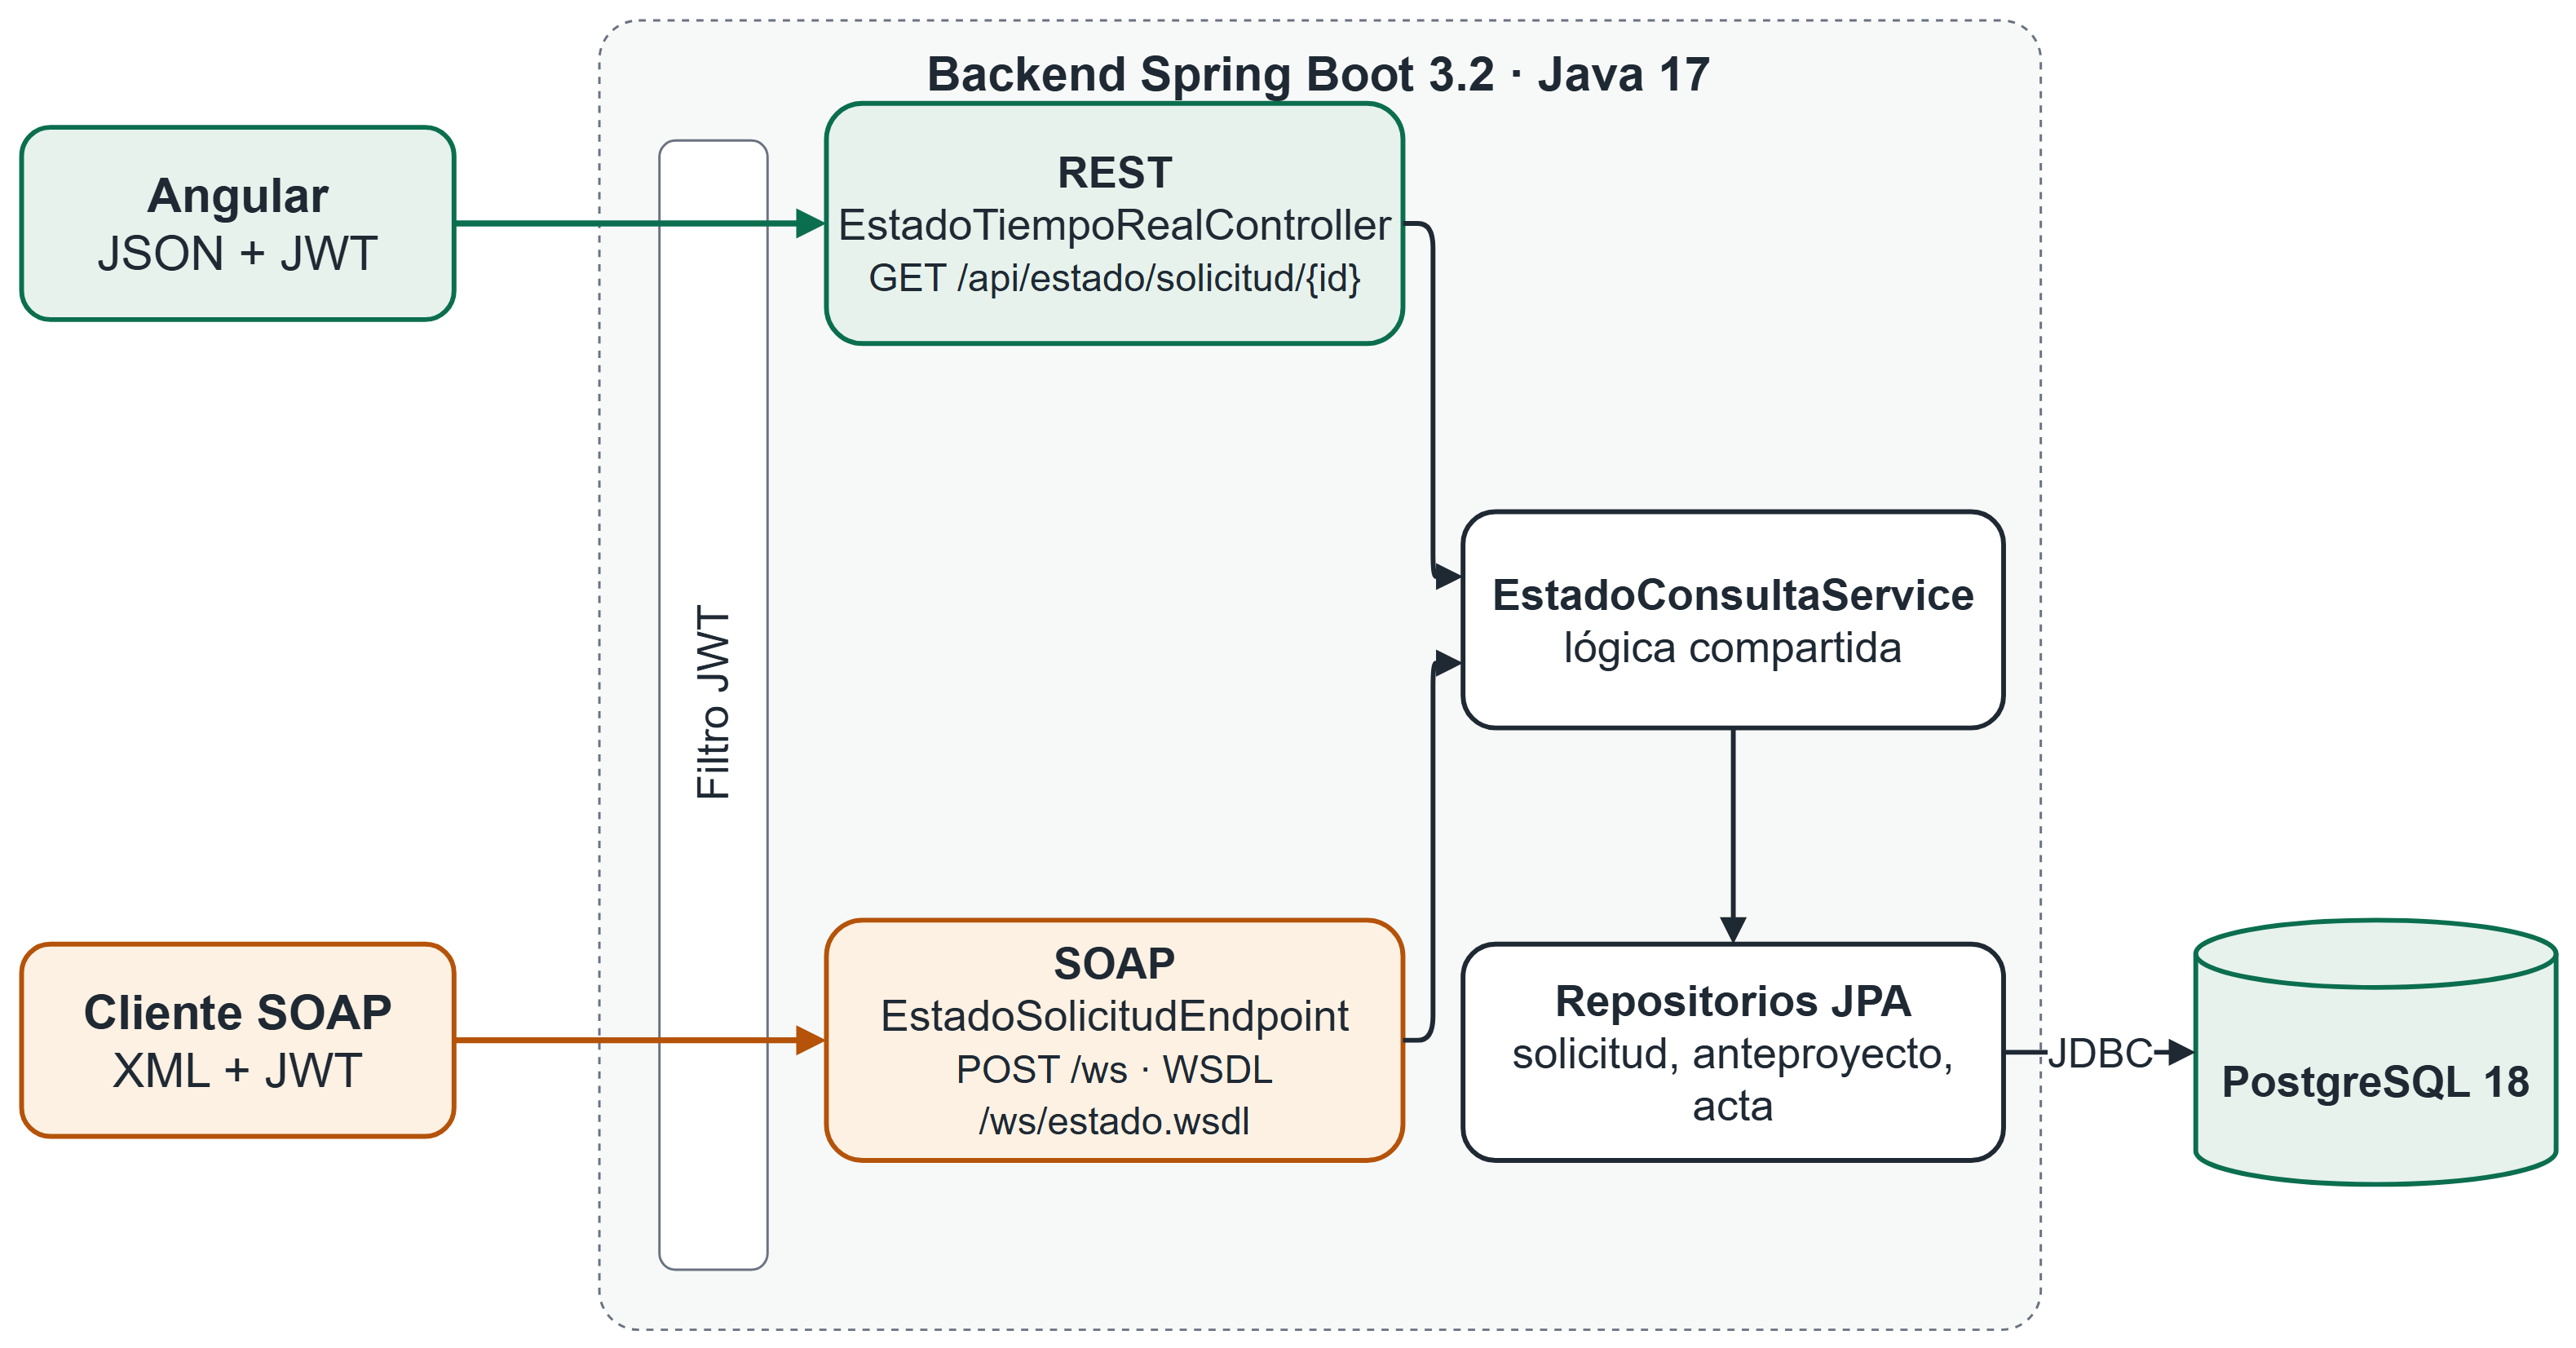
\includegraphics[width=0.94\linewidth,height=0.72\textheight,keepaspectratio]{../diagrama/arquitectura-servicios-web.png}}{\fbox{\parbox[c][4cm][c]{0.8\linewidth}{\centering\color{gris}Falta \texttt{diagrama/arquitectura-servicios-web.png}}}}
\par\vspace{4pt}
{\footnotesize Diagrama propio en draw.io: el mismo servicio de negocio se ofrece por REST y por SOAP.\par}
\end{frame}
